\documentclass[dvipdfmx]{jsarticle}
\usepackage{amsfonts}
\usepackage{amsmath}
\usepackage{here}
\usepackage{physics}
\usepackage{tikz}
\usetikzlibrary{angles}
\makeatletter
\newcommand{\subsubsubsection}{\@startsection{paragraph}{4}{\z@}%
 {1.0\Cvs \@plus.5\Cdp \@minus.2\Cdp}%
 {.1\Cvs \@plus.3\Cdp}%
 {\reset@font\sffamily\normalsize}
}
\makeatother
\setcounter{secnumdepth}{4}
\title{微積分}
\author{伊藤 太清}
\date{\today}
\begin{document}
 \maketitle
 \tableofcontents
 \section{微分}
  \subsection{定義}
   \begin{align}
    \dv{f\left(x\right)}{x}=\lim_{h\to 0}\frac{f\left(x+h\right)-f\left(x\right)}{h}
   \end{align}
  \subsection{定数の微分}
   \begin{align}
    f\left(x\right)=a
   \end{align}
   のとき,
   \begin{align}
    \dv{f\left(x\right)}{x}&=\lim_{h\to 0}\frac{f\left(x+h\right)-f\left(x\right)}{h}\nonumber\\
    &=\lim_{h\to 0}\frac{a-a}{h}\nonumber\\
    &=\lim_{h\to 0}\frac{0}{h}\nonumber\\
    &=\lim_{h\to 0}0\nonumber\\
    &=0
   \end{align}
  \subsection{恒等関数の微分}
   \begin{align}
    f\left(x\right)=x
   \end{align}
   のとき,
   \begin{align}
    \dv{f\left(x\right)}{x}&=\lim_{h\to 0}\frac{f\left(x+h\right)-f\left(x\right)}{h}\nonumber\\
    &=\lim_{h\to 0}\frac{x+h-x}{h}\nonumber\\
    &=\lim_{h\to 0}\frac{h}{h}\nonumber\\
    &=\lim_{h\to 0}1\nonumber\\
    &=1
   \end{align}
  \subsection{逆数の微分}
   \begin{align}
    f\left(x\right)=\frac{1}{x}
   \end{align}
   のとき,
   \begin{align}
    \dv{f\left(x\right)}{x}&=\lim_{h\to 0}\frac{f\left(x+h\right)-f\left(x\right)}{h}\nonumber\\
    &=\lim_{h\to 0}\frac{\frac{1}{x+h}-\frac{1}{x}}{h}\nonumber\\
    &=\lim_{h\to 0}\frac{\frac{x}{x\left(x+h\right)}-\frac{x+h}{x\left(x+h\right)}}{h}\nonumber\\
    &=\lim_{h\to 0}\frac{x-x-h}{hx\left(x+h\right)}\nonumber\\
    &=\lim_{h\to 0}-\frac{h}{hx\left(x+h\right)}\nonumber\\
    &=\lim_{h\to 0}-\frac{1}{x\left(x+h\right)}\nonumber\\
    &=-\frac{1}{x^2}
   \end{align}
  \subsection{指数関数の微分}
   \subsubsection{有理数の実数への拡張}
    $\mathbb{Q}$のデデキント切断とは,以下が成り立つように$\mathbb{Q}$を$\mathbb{Q}_{<x}$と${}_{x\le}\mathbb{Q}$に切断することである.
    \begin{align}
     &\mathbb{Q}_{<x}\ne\emptyset\\
     &{}_{x\le}\mathbb{Q}\ne\emptyset\\
     &\mathbb{Q}_{<x}\cup{}_{x\le}\mathbb{Q}=\mathbb{Q}\\
     &\mathbb{Q}_{<x}\cap{}_{x\le}\mathbb{Q}=\emptyset\\
     &\forall q\in\mathbb{Q}_{<x},\exists r\in\mathbb{Q}_{<x},q<r
    \end{align}
    デデキント切断において,
    \begin{align}
     \exists x\in{}_{x\le}\mathbb{Q},\forall q\in{}_{x\le}\mathbb{Q},x\le q
    \end{align}
    が成り立つ場合と成り立たない場合がある.
    成り立つ場合,$x\in\mathbb{Q}$だが,成り立たない場合,$x\in\mathbb{R}-\mathbb{Q}$である.
    つまり,デデキント切断は有理数から無理数を生み出す能力を持つ.
    例えば,
    \begin{align}
     \mathbb{Q}_{<\sqrt{2}}&=\{q\in\mathbb{Q}|q<0\lor q^2<2\}\\
     {}_{\sqrt{2}\le}\mathbb{Q}&=\{q\in\mathbb{Q}|0\le q\land 2\le q^2\}
    \end{align}
    において${}_{\sqrt{2}\le}\mathbb{Q}$は最小値を持たない.
    このデデキント切断における$\mathbb{Q}$上に存在しない最小値は$\sqrt{2}\in\mathbb{R}-\mathbb{Q}$と定義される.
   \subsubsection{$\mathbb{R}$上の順序関係の定義}
    \begin{align}
     \forall\left(a,b\right)\in\mathbb{R}^2,a<b\iff\mathbb{Q}_{<a}\subset\mathbb{Q}_{<b}\\
     \forall\left(a,b\right)\in\mathbb{R}^2,a\le b\iff\mathbb{Q}_{<a}\subseteq\mathbb{Q}_{<b}\\
     \forall\left(a,b\right)\in\mathbb{R}^2,a=b\iff\mathbb{Q}_{<a}=\mathbb{Q}_{<b}
    \end{align}
   \subsubsection{上界,下界の定義}
    上界$R\le u$の定義は以下の通りである.
    \begin{align}
     \forall \left(R, u\right)\in 2^\mathbb{R}\times\mathbb{R},R\le u\iff\forall r\in R,r\le u
    \end{align}
    下界$l\le R$の定義は以下の通りである.
    \begin{align}
     \forall \left(R, l\right)\in 2^\mathbb{R}\times\mathbb{R},l\le R\iff\forall r\in R,l\le r
    \end{align}
   \subsubsection{上限,下限の定義}
    \begin{align}
     {}_{0<}\mathbb{R}=\{x\in\mathbb{R}|0<x\}
    \end{align}
    とする.
    $\forall R\subset\mathbb{R}$の上限$\sup R$は以下を満たす.
    \begin{align}
     \forall R\subset\mathbb{R},R\le\sup R\land\forall\epsilon\in{}_{0<}\mathbb{R},R\cap\left[\sup R-\epsilon,\sup R\right]\ne\emptyset
    \end{align}
    $\forall R\subset\mathbb{R}$の下限$\inf R$は以下を満たす.
    \begin{align}
     \forall R\subset\mathbb{R},\inf R\le R\land\forall\epsilon\in{}_{0<}\mathbb{R},R\cap\left[\inf R,\inf R+\epsilon\right]\ne\emptyset
    \end{align}
   \subsubsection{実数の連続性}
    上界$u$を持つ$\emptyset\ne\forall R\subset\mathbb{R}$は,必ず上限$\sup R$を持つことを証明する.
    まず,
    \begin{align}
     \mathbb{Q}_{<x}&=\bigcup_{r\in R}\mathbb{Q}_{<r}\\
     {}_{x\le}\mathbb{Q}=\mathbb{Q}-\mathbb{Q}_{<x}&=\bigcap_{r\in R}{}_{r\le}\mathbb{Q}
    \end{align}
    がデデキント切断であることを証明し,その後,$x=\sup R$を証明する.
    \subsubsubsection{デデキント切断であることの証明}
     $R\ne\emptyset$より,$\exists r\in R$で,$\mathbb{Q}_{<r}\subset\mathbb{Q}_{<\sup R}\ne\emptyset$である.
     $R\le u$より,$\forall r\in R,r\le u$で,$u\in{}_{x\le}\mathbb{Q}\ne\emptyset$である.
     $\mathbb{Q}_{<x}\cup{}_{x\le}\mathbb{Q}$は全て$\mathbb{Q}$の部分集合で構成されているから$\mathbb{Q}_{<x}\cup{}_{x\le}\mathbb{Q}\subset\mathbb{Q}$である.
     $\forall q\in\mathbb{Q}$について,$q\in\mathbb{Q}_{<x}$さもなくば$q\in{}_{x\le}\mathbb{Q}$であるから,$\mathbb{Q}\subset\mathbb{Q}_{<x}\cup{}_{x\le}\mathbb{Q}$である.
     よって$\mathbb{Q}_{<x}\cup{}_{x\le}\mathbb{Q}=\mathbb{Q}$である.
     $\forall q\in\mathbb{Q}_{<x}$について,$\exists r\in R,q\in\mathbb{Q}_{<r}$であり,$r\in\mathbb{R}$より$\mathbb{Q}_{<r}$と${}_{r\le}\mathbb{Q}$はデデキント切断であるから$\exists s\in\mathbb{Q}_{<r}\subset\mathbb{Q}_{<x},q<s$である.
     以上より$\mathbb{Q}_{<x}$と${}_{x\le}\mathbb{Q}$はデデキント切断となっており,$\exists x\in\mathbb{R}$である.
    \subsubsubsection{$R\le x$の証明}
     $\forall r\in R$について,$\mathbb{Q}_{<r}\subseteq\mathbb{Q}_{<x}$よって$r\le x$よって$R\le x$
    \subsubsubsection{$x=\sup R$の証明}
     $R\le\forall y$について,$\forall r\in R$について,$r\le y$よって$\mathbb{Q}_{<r}\subseteq\mathbb{Q}_{<y}$よって${}_{y\le}\mathbb{Q}\subseteq{}_{r\le}\mathbb{Q}$よって${}_{y\le}\mathbb{Q}\subseteq{}_{x\le}\mathbb{Q}$よって$\mathbb{Q}_{<x}\subseteq\mathbb{Q}_{<y}$よって$x\le y$よって$x=\sup R$
   \subsubsection{単調収束定理}
    単調増加数列
    \begin{align}
     &f:\mathbb{N}\to\mathbb{R}\\
     &\forall n\in\mathbb{N},f\left(n\right)\le f\left(n+1\right)
    \end{align}
    の像$f\left(\mathbb{N}\right)$が,上界を持つとき,上限$\sup f\left(\mathbb{N}\right)$が存在するので,$\forall\epsilon\in{}_{0<}\mathbb{R}$について,
    \begin{align}
     &f\left(\mathbb{N}\right)\cap\left[\sup f\left(\mathbb{N}\right)-\epsilon,\sup f\left(\mathbb{N}\right)\right]\ne\emptyset\nonumber\\
     &\iff\exists n\in\mathbb{N},\sup f\left(\mathbb{N}\right)-\epsilon\le f\left(n\right)\le\sup f\left(\mathbb{N}\right)\nonumber\\
     &\iff\exists n\in\mathbb{N},0\le\sup f\left(\mathbb{N}\right)-f\left(n\right)\le\epsilon
    \end{align}
    さらに単調増加性より,
    \begin{align}
     &\forall\epsilon\in{}_{0<}\mathbb{R},\exists n\in\mathbb{N},\forall m\in{}_{n\le}\mathbb{N},0\le\sup f\left(\mathbb{N}\right)-f\left(m\right)\le\epsilon\nonumber\\
     &\iff\lim_{n\to\infty}f\left(n\right)=\sup f\left(\mathbb{N}\right)
    \end{align}
   \subsubsection{ボルツァーノ・ワイエルシュトラスの定理}
    有界な数列が収束する部分列を持つことを証明する.
    数列
    \begin{align}
     f:\mathbb{N}\to\left[\min f\left(\mathbb{N}\right),\max f\left(\mathbb{N}\right)\right]
    \end{align}
    に対して,性質
    \begin{align}
     g:\mathbb{N}\to\{\top,\bot\};n\mapsto\forall m\in{}_{n<}\mathbb{N},f\left(m\right)<f\left(n\right)
    \end{align}
    の逆像の濃度
    \begin{align}
     \left|g^{-1}\left(\top\right)\right|
    \end{align}
    が,$0$の場合,有限個の場合,可算無限個の場合に分けて考える.
    \subsubsubsection{$\left|g^{-1}\left(\top\right)\right|=0$の場合}
     \begin{align}
      &\forall n\in\mathbb{N},\lnot g\left(n\right)\nonumber\\
      &\iff\forall n\in\mathbb{N},\lnot \forall m\in{}_{n<}\mathbb{N},f\left(m\right)<f\left(n\right)\nonumber\\
      &\iff\forall n\in\mathbb{N},\exists m\in{}_{n<}\mathbb{N},\lnot f\left(m\right)<f\left(n\right)\nonumber\\
      &\iff\forall n\in\mathbb{N},\exists m\in{}_{n<}\mathbb{N},f\left(n\right)\le f\left(m\right)
     \end{align}
     よって単調増加な部分列が存在する.
    \subsubsubsection{$\left|g^{-1}\left(\top\right)\right|<\aleph_0$の場合}
     \begin{align}
      &\left|g^{-1}\left(\top\right)\right|<\aleph_0\nonumber\\
      &\iff \max g^{-1}\left(\top\right)
     \end{align}
     よって部分列
     \begin{align}
      f_1:\mathbb{N}\to\mathbb{R};n\mapsto f\left(n+\max g^{-1}\left(\top\right)\right)
     \end{align}
     は,性質
     \begin{align}
      g_1:\mathbb{N}\to\{\top,\bot\};n\mapsto\forall m\in{}_{n<}\mathbb{N},f_1\left(m\right)<f_1\left(n\right)
     \end{align}
     について,
     \begin{align}
      &\forall n\in\mathbb{N},\max g^{-1}\left(\top\right)<n+\max g^{-1}\left(\top\right)\nonumber\\
      &\implies\forall n\in\mathbb{N},\lnot g\left(n+\max g^{-1}\left(\top\right)\right)\nonumber\\
      &\iff\forall n\in\mathbb{N},\lnot\forall k\in{}_{n+\max g^{-1}\left(\top\right)<}\mathbb{N},f\left(k\right)<f\left(n+\max g^{-1}\left(\top\right)\right)\nonumber\\
      &\iff\forall n\in\mathbb{N},\exists k\in{}_{n+\max\left(g^{-1}\left(\top\right)\right)<}\mathbb{N},\lnot f\left(k\right)<f\left(n+\max g^{-1}\left(\top\right)\right)\nonumber\\
      &\iff\forall n\in\mathbb{N},\exists k\in{}_{n+\max\left(g^{-1}\left(\top\right)\right)<}\mathbb{N},f\left(n+\max g^{-1}\left(\top\right)\right)\le f\left(k\right)\nonumber\\
      &\iff\forall n\in\mathbb{N},\exists k\in{}_{n<}\mathbb{N},f_1\left(n\right)\le f_1\left(k\right)\nonumber\\
      &\iff\forall n\in\mathbb{N},\exists k\in{}_{n<}\mathbb{N},\lnot f_1\left(k\right)<f_1\left(n\right)\nonumber\\
      &\iff\forall n\in\mathbb{N},\lnot\forall k\in{}_{n<}\mathbb{N},f_1\left(k\right)<f_1\left(n\right)\nonumber\\
      &\iff\forall n\in\mathbb{N},\lnot g_1\left(n\right)\nonumber\\
      &\iff\left|g_1^{-1}\left(\top\right)\right|=0
     \end{align}
     よって部分列$f_1$は単調増加な部分列を持つ.
    \subsubsubsection{$\left|g^{-1}\left(\top\right)\right|=\aleph_0$の場合}
     部分列
     \begin{align}
      f_1:g^{-1}\left(\top\right)\to\left[\min f\left(\mathbb{N}\right),\max f\left(\mathbb{N}\right)\right];n\mapsto f\left(n\right)
     \end{align}
     は,
     \begin{align}
      &\forall n\in g^{-1}\left(\top\right),g\left(n\right)\nonumber\\
      &\iff\forall n\in g^{-1}\left(\top\right),\forall m\in{}_{n<}\mathbb{N},f\left(m\right)<f\left(n\right)\nonumber\\
      &\implies\forall n\in g^{-1}\left(\top\right),\forall m\in{}_{n<}g^{-1}\left(\top\right),f_1\left(m\right)<f_1\left(n\right)
     \end{align}
     より,単調減少である.
   \subsubsection{相加相乗平均の不等式}
    \begin{align}
     \forall n\in\mathbb{N},\forall s\in{}_{0\le}\mathbb{R}^{\mathbb{N}_{\le n}},\left(\prod_{i=1}^ns\left(i\right)\right)^{n^{-1}}\le n^{-1}\sum_{i=1}^ns\left(i\right)
    \end{align}
    を証明する.
    \begin{align}
     p:\mathbb{N}\to\{\top,\bot\};n\mapsto\forall s\in{}_{0\le}\mathbb{R}^{\mathbb{N}_{\le n}},\left(\prod_{i=1}^ns\left(i\right)\right)^{n^{-1}}\le n^{-1}\sum_{i=1}^ns\left(i\right)
    \end{align}
    とし,
    \begin{align}
     &p\left(1\right)\\
     &p\left(2^n\right)\implies p\left(2^{n+1}\right)\\
     &p\left(n+1\right)\implies p\left(n\right)
    \end{align}
    をそれぞれ証明すれば,
    \begin{align}
     \forall n\in\mathbb{N},p\left(n\right)
    \end{align}
    といえる.
    \subsubsubsection{$p\left(1\right)$}
     自明
    \subsubsubsection{$p\left(2^n\right)\implies p\left(2^{n+1}\right)$}
     \begin{align}
      2^{-n-1}\sum_{i=1}^{2^{n+1}}s\left(i\right)&=2^{-1}\left(2^{-n}\sum_{i=1}^{2^n}s\left(i\right)+2^{-n}\sum_{i=2^n+1}^{2^{n+1}}s\left(i\right)\right)\nonumber\\
      &\ge2^{-1}\left(\left(\prod_{i=1}^{2^n}s\left(i\right)\right)^{2^{-n}}+\left(\prod_{i=2^n+1}^{2^{n+1}}s\left(i\right)\right)^{2^{-n}}\right)\nonumber\\
      &\ge\left(\left(\prod_{i=1}^{2^n}s\left(i\right)\right)^{2^{-n}}\left(\prod_{i=2^n+1}^{2^{n+1}}s\left(i\right)\right)^{2^{-n}}\right)^{2^{-1}}\nonumber\\
      &=\left(\left(\prod_{i=1}^{2^{n+1}}s\left(i\right)\right)^{2^{-n}}\right)^{2^{-1}}\nonumber\\
      &=\left(\prod_{i=1}^{2^{n+1}}s\left(i\right)\right)^{2^{-n-1}}
     \end{align}
    \subsubsubsection{$p\left(n+1\right)\implies p\left(n\right)$}
   \subsubsection{自然対数の底の定義}
    \begin{align}
     e=\lim_{n\to\infty}\left(1+\frac{1}{n}\right)^n
    \end{align}
   \subsubsection{自然対数の底の収束性}
   \subsubsection{自然対数の底の無理性}
   \subsubsection{指数関数と対数関数の極限の公式}
   \subsubsection{本証明}
    自然対数の底の定義
    \begin{align}
     e&=\lim_{x\to\infty}\left(1+\frac{1}{x}\right)^x\nonumber\\
     &=\lim_{h\to 0}\left(1+h\right)^{\frac{1}{h}}
    \end{align}
    より,
    \begin{align}
     \dv{e^x}{x}&=\lim_{h\to 0}\frac{e^{x+h}-e^x}{h}\nonumber\\
     &=\lim_{h\to 0}\frac{e^xe^h-e^x}{h}\nonumber\\
     &=\lim_{h\to 0}\frac{e^x\left(e^h-1\right)}{h}\nonumber\\
     &=e^x\lim_{h\to 0}\frac{e^h-1}{h}\nonumber\\
     &=e^x\lim_{h\to 0}\frac{\left(\left(1+h\right)^{\frac{1}{h}}\right)^h-1}{h}\nonumber\\
     &=e^x\lim_{h\to 0}\frac{\left(1+h\right)^{\frac{h}{h}}-1}{h}\nonumber\\
     &=e^x\lim_{h\to 0}\frac{\left(1+h\right)-1}{h}\nonumber\\
     &=e^x\lim_{h\to 0}\frac{h}{h}\nonumber\\
     &=e^x\lim_{h\to 0}1\nonumber\\
     &=e^x
    \end{align}
  \subsection{対数関数の微分}
   \begin{align}
    \dv{\log x}{x}&=\lim_{h\to 0}\frac{\log\left(x+h\right)-\log x}{h}\nonumber\\
    &=\lim_{h\to 0}\frac{\log\frac{x+h}{x}}{h}\nonumber\\
    &=\lim_{h\to 0}\log\left(\frac{x+h}{x}\right)^{\frac{1}{h}}\nonumber\\
    &=\log\lim_{h\to 0}\left(\frac{x}{x}+\frac{h}{x}\right)^{\frac{1}{h}}\nonumber\\
    &=\log\lim_{h\to 0}\left(1+\frac{h}{x}\right)^{\frac{1}{h}}
   \end{align}
   ここで,
   \begin{align}
    g=\frac{h}{x}
   \end{align}
   とすると,
   \begin{align}
    \dv{\log x}{x}&=\log\lim_{h\to 0}\left(1+\frac{h}{x}\right)^{\frac{1}{h}}\nonumber\\
    &=\log\lim_{g\to 0}\left(1+g\right)^{\frac{1}{gx}}\nonumber\\
    &=\log\lim_{g\to 0}\left(\left(1+g\right)^{\frac{1}{g}}\right)^{\frac{1}{x}}\nonumber\\
    &=\log\left(\lim_{g\to 0}\left(1+g\right)^{\frac{1}{g}}\right)^{\frac{1}{x}}\nonumber\\
    &=\log e^{\frac{1}{x}}\nonumber\\
    &=\frac{1}{x}\nonumber\\
   \end{align}
  \subsection{$\sin$の微分}
   \subsubsection{三平方の定理}
    \begin{figure}[H]
     \begin{center}
      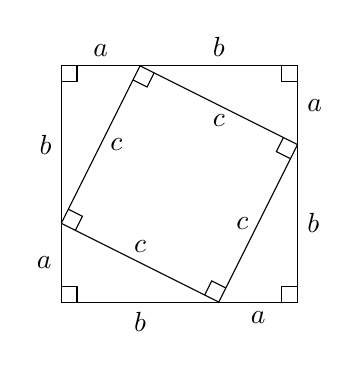
\begin{tikzpicture}
       \coordinate(BottomLeft)at(0,0);
       \coordinate(Left)at(0,1);
       \coordinate(TopLeft)at(0,3);
       \coordinate(Top)at(1,3);
       \coordinate(TopRight)at(3,3);
       \coordinate(Right)at(3,2);
       \coordinate(BottomRight)at(3,0);
       \coordinate(Bottom)at(2,0);
       \draw(TopLeft)--(Top)node[midway, above]{$a$};
       \draw(Top)--(TopRight)node[midway, above]{$b$};
       \draw(TopRight)--(Right)node[midway, right]{$a$};
       \draw(Right)--(BottomRight)node[midway, right]{$b$};
       \draw(BottomRight)--(Bottom)node[midway, below]{$a$};
       \draw(Bottom)--(BottomLeft)node[midway, below]{$b$};
       \draw(BottomLeft)--(Left)node[midway, left]{$a$};
       \draw(Left)--(TopLeft)node[midway, left]{$b$};
       \pic[draw,angle radius=2mm]{right angle=TopLeft--TopRight--BottomRight};
       \pic[draw,angle radius=2mm]{right angle=TopRight--BottomRight--BottomLeft};
       \pic[draw,angle radius=2mm]{right angle=BottomRight--BottomLeft--TopLeft};
       \pic[draw,angle radius=2mm]{right angle=BottomLeft--TopLeft--TopRight};
       \draw(Top)--(Right)node[midway, below]{$c$};
       \draw(Right)--(Bottom)node[midway, left]{$c$};
       \draw(Bottom)--(Left)node[midway, above]{$c$};
       \draw(Left)--(Top)node[midway, right]{$c$};
       \pic[draw,angle radius=2mm]{right angle=Top--Right--Bottom};
       \pic[draw,angle radius=2mm]{right angle=Right--Bottom--Left};
       \pic[draw,angle radius=2mm]{right angle=Bottom--Left--Top};
       \pic[draw,angle radius=2mm]{right angle=Left--Top--Right};
      \end{tikzpicture}
     \end{center}
     \caption{三平方の定理の証明}
    \end{figure}
    \begin{align}
     \left(a+b\right)^2&=c^2+4\frac{ab}{2}\nonumber\\
     a^2+2ab+b^2&=c^2+2ab\nonumber\\
     a^2+b^2&=c^2
    \end{align}
   \subsubsection{余弦定理}
    $\triangle ABC$があり,頂点$A$から辺$BC$へ垂線を引き,その足を点$D$とする.
    \begin{figure}[H]
     \begin{center}
      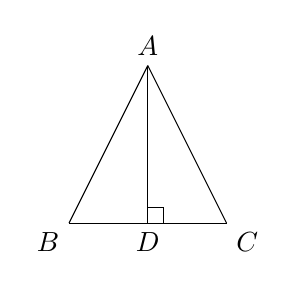
\begin{tikzpicture}
       \coordinate(A)at(1,2);
       \coordinate(B)at(0,0);
       \coordinate(C)at(2,0);
       \coordinate(D)at(1,0);
       \node[above]at(A){$A$};
       \node[below left]at(B){$B$};
       \node[below right]at(C){$C$};
       \node[below]at(D){$D$};
       \draw(A)--(B);
       \draw(B)--(C);
       \draw(C)--(A);
       \draw(A)--(D);
       \pic[draw,angle radius=2mm]{right angle=A--D--C};
      \end{tikzpicture}
     \end{center}
     \caption{$\triangle ABC$}
    \end{figure}
    直角三角形$\triangle ABD$について,三平方の定理より,
    \begin{align}
     \left|\vec{AD}\right|^2+\left|\vec{BD}\right|^2&=\left|\vec{AB}\right|^2\nonumber\\
     \left|\vec{AD}\right|^2&=\left|\vec{AB}\right|^2-\left|\vec{BD}\right|^2
    \end{align}
    また,直角三角形$\triangle ACD$について,三平方の定理より,
    \begin{align}
     \left|\vec{AD}\right|^2+\left|\vec{CD}\right|^2&=\left|\vec{AC}\right|^2\nonumber\\
     \left|\vec{AD}\right|^2&=\left|\vec{AC}\right|^2-\left|\vec{CD}\right|^2
    \end{align}
    よって,
    \begin{align}
     \left|\vec{AB}\right|^2-\left|\vec{BD}\right|^2&=\left|\vec{AD}\right|^2=\left|\vec{AC}\right|^2-\left|\vec{CD}\right|^2\nonumber\\
     \left|\vec{AB}\right|^2-\left|\vec{BD}\right|^2&=\left|\vec{AC}\right|^2-\left|\vec{CD}\right|^2\nonumber\\
     \left|\vec{AB}\right|^2-\left|\vec{BD}\right|^2&=\left|\vec{AC}\right|^2-\left(\left|\vec{BC}\right|-\left|\vec{BD}\right|\right)^2\nonumber\\
     \left|\vec{AB}\right|^2-\left(\left|\vec{AB}\right|\cos\angle ABC\right)^2&=\left|\vec{AC}\right|^2-\left(\left|\vec{BC}\right|-\left|\vec{AB}\right|\cos\angle ABC\right)^2\nonumber\\
     \left|\vec{AB}\right|^2-\left|\vec{AB}\right|^2\cos^2\angle ABC&=\left|\vec{AC}\right|^2-\left(\left|\vec{BC}\right|^2-2\left|\vec{BC}\right|\left|\vec{AB}\right|\cos\angle ABC+\left|\vec{AB}\right|^2\cos^2\angle ABC\right)\nonumber\\
     \left|\vec{AB}\right|^2-\left|\vec{AB}\right|^2\cos^2\angle ABC&=\left|\vec{AC}\right|^2-\left|\vec{BC}\right|^2+2\left|\vec{BC}\right|\left|\vec{AB}\right|\cos\angle ABC-\left|\vec{AB}\right|^2\cos^2\angle ABC\nonumber\\
     \left|\vec{AB}\right|^2&=\left|\vec{AC}\right|^2-\left|\vec{BC}\right|^2+2\left|\vec{BC}\right|\left|\vec{AB}\right|\cos\angle ABC\nonumber\\
     \left|\vec{AB}\right|^2+\left|\vec{BC}\right|^2-\left|\vec{AC}\right|^2&=2\left|\vec{AB}\right|\left|\vec{BC}\right|\cos\angle ABC
    \end{align}
   \subsubsection{加法定理}
    \begin{figure}[H]
     \begin{center}
      \begin{tikzpicture}
       \pgfmathsetmacro{\a}{30};
       \pgfmathsetmacro{\b}{60};
       \coordinate(O)at(0,0);
       \coordinate(Xn)at(-3,0);
       \coordinate(Xp)at(3,0);
       \coordinate(Yn)at(0,-3);
       \coordinate(Yp)at(0,3);
       \coordinate(A)at({3*cos(\a)},{3*sin(\a)});
       \coordinate(B)at({3*cos(\b)},{3*sin(\b)});
       \node[below left]at(O){$O$};
       \node[above right]at(A){$A$};
       \node[above right]at(B){$B$};
       \node[right]at(Xp){$X$};
       \node[above]at(Yp){$Y$};
       \draw(Xn)--(Xp);
       \draw(Yn)--(Yp);
       \draw(O)--(A);
       \draw(O)--(B);
       \draw([shift={(O)}]\a:3)arc[radius=3,start angle={\a},end angle={\b}];
       \draw([shift={(O)}]0:1)arc[radius=1,start angle=0,end angle={\b}]node[right]{$\beta$};
       \draw([shift={(O)}]0:2)arc[radius=2,start angle=0,end angle={\a}]node[right]{$\alpha$};
      \end{tikzpicture}
     \end{center}
     \caption{加法定理}
    \end{figure}
    原点$O=\left(0,0\right)$,点$A=\left(\cos\alpha,\sin\alpha\right)$,点$B=\left(\cos\beta,\sin\beta\right)$とすると,$\triangle OAB$について,余弦定理より,
    \begin{align}
     2\left|\vec{OA}\right|\left|\vec{OB}\right|\cos\angle AOB&=\left|\vec{OA}\right|^2+\left|\vec{OB}\right|^2-\left|\vec{AB}\right|^2\nonumber\\
     2\cos\left(\alpha-\beta\right)&=1+1-\left(\left(\cos\alpha-\cos\beta\right)^2+\left(\sin\alpha-\sin\beta\right)^2\right)\nonumber\\
     2\cos\left(\alpha-\beta\right)&=2-\left(\cos^2\alpha-2\cos\alpha\cos\beta+\cos^2\beta+\sin^2\alpha-2\sin\alpha\sin\beta+\sin^2\beta\right)\nonumber\\
     2\cos\left(\alpha-\beta\right)&=2-\left(\left(\sin^2\alpha+\cos^2\alpha\right)+\left(\sin^2\beta+\cos^2\beta\right)-2\cos\alpha\cos\beta-2\sin\alpha\sin\beta\right)\nonumber\\
     2\cos\left(\alpha-\beta\right)&=2-\left(1+1-2\cos\alpha\cos\beta-2\sin\alpha\sin\beta\right)\nonumber\\
     2\cos\left(\alpha-\beta\right)&=2-\left(2-2\cos\alpha\cos\beta-2\sin\alpha\sin\beta\right)\nonumber\\
     2\cos\left(\alpha-\beta\right)&=2-2+2\cos\alpha\cos\beta+2\sin\alpha\sin\beta\nonumber\\
     2\cos\left(\alpha-\beta\right)&=2\cos\alpha\cos\beta+2\sin\alpha\sin\beta\nonumber\\
     \cos\left(\alpha-\beta\right)&=\cos\alpha\cos\beta+\sin\alpha\sin\beta
    \end{align}
    $\beta$を$-\beta$に変えると,
    \begin{align}
     \cos\left(\alpha-\left(-\beta\right)\right)&=\cos\alpha\cos\left(-\beta\right)+\sin\alpha\sin\left(-\beta\right)\nonumber\\
     \cos\left(\alpha+\beta\right)&=\cos\alpha\cos\beta-\sin\alpha\sin\beta
    \end{align}
    また,
    \begin{align}
     \sin\left(\alpha+\beta\right)&=\cos\left(\alpha+\beta-\frac{\pi}{2}\right)\nonumber\\
     &=\cos\alpha\cos\left(\beta-\frac{\pi}{2}\right)-\sin\alpha\sin\left(\beta-\frac{\pi}{2}\right)\nonumber\\
     &=\cos\alpha\sin\beta-\sin\alpha\left(-\cos\beta\right)\nonumber\\
     &=\cos\alpha\sin\beta+\sin\alpha\cos\beta\nonumber\\
     &=\sin\alpha\cos\beta+\cos\alpha\sin\beta
    \end{align}
    まとめると,
    \begin{align}
     \begin{pmatrix}
      \cos\left(\alpha+\beta\right)\\
      \sin\left(\alpha+\beta\right)
     \end{pmatrix}&=
     \begin{pmatrix}
      \cos\beta&-\sin\beta\\
      \sin\beta&\cos\beta
     \end{pmatrix}
     \begin{pmatrix}
      \cos\alpha\\
      \sin\alpha
     \end{pmatrix}
    \end{align}
   \subsubsection{$\sin$の極限}
    正無限角形の周の長さと,円周の長さは等しいので,
    \begin{align}
     \lim_{n\to\infty}2n\sin\frac{\pi}{n}&=2\pi\nonumber\\
     \lim_{n\to\infty}\frac{n}{\pi}\sin\frac{\pi}{n}&=1\nonumber\\
     \lim_{\theta\to 0}\frac{\sin\theta}{\theta}&=1
    \end{align}
   \subsubsection{$\cos$の極限}
    \begin{align}
     \lim_{\theta\to 0}\frac{\sin\theta}{\theta}&=1\nonumber\\
     \lim_{\theta\to 0}\frac{\sin^2\theta}{\theta^2}&=1\nonumber\\
     \lim_{\theta\to 0}\frac{1-\cos^2\theta}{\theta^2}&=1\nonumber\\
     \lim_{\theta\to 0}\frac{\left(1-\cos\theta\right)\left(1+\cos\theta\right)}{\theta^2}&=1\nonumber\\
     \left(\lim_{\theta\to 0}\frac{1-\cos\theta}{\theta^2}\right)\left(\lim_{\theta\to 0}\left(1+\cos\theta\right)\right)&=1\nonumber\\
     \left(\lim_{\theta\to 0}\frac{1-\cos\theta}{\theta^2}\right)\left(1+\lim_{\theta\to 0}\cos\theta\right)&=1\nonumber\\
     \left(\lim_{\theta\to 0}\frac{1-\cos\theta}{\theta^2}\right)\left(1+1\right)&=1\nonumber\\
     \left(\lim_{\theta\to 0}\frac{1-\cos\theta}{\theta^2}\right)2&=1\nonumber\\
     \lim_{\theta\to 0}\frac{1-\cos\theta}{\theta^2}&=\frac{1}{2}\nonumber\\
    \end{align}
   \subsubsection{本証明}
    \begin{align}
     \dv{\sin x}{x}&=\lim_{h\to 0}\frac{\sin\left(x+h\right)-\sin x}{h}\nonumber\\
     &=\lim_{h\to 0}\frac{\sin x\cos h +\cos x\sin h-\sin x}{h}\nonumber\\
     &=\lim_{h\to 0}\frac{\sin x\left(\cos h-1\right) +\cos x\sin h}{h}\nonumber\\
     &=\lim_{h\to 0}\sin x\frac{\cos h-1}{h} +\cos x\frac{\sin h}{h}\nonumber\\
     &=\lim_{h\to 0}h\frac{\cos h-1}{h^2}\sin x +\frac{\sin h}{h}\cos x\nonumber\\
     &=\left(\lim_{h\to 0}h\right)\left(\lim_{h\to 0}\frac{\cos h-1}{h^2}\right)\sin x +\left(\lim_{h\to 0}\frac{\sin h}{h}\right)\cos x\nonumber\\
     &=0\left(-\frac{1}{2}\right)\sin x +1\cos x\nonumber\\
     &=\cos x
    \end{align}
  \subsection{$\cos$の微分}
   \begin{align}
    \dv{\cos x}{x}&=\lim_{h\to 0}\frac{\cos\left(x+h\right)-\cos x}{h}\nonumber\\
    &=\lim_{h\to 0}\frac{\cos x\cos h-\sin x\sin h-\cos x}{h}\nonumber\\
    &=\lim_{h\to 0}\frac{\cos x\left(\cos h - 1\right)-\sin x\sin h}{h}\nonumber\\
    &=\lim_{h\to 0}\cos x\frac{\cos h - 1}{h}-\sin x\frac{\sin h}{h}\nonumber\\
    &=\lim_{h\to 0}h\frac{\cos h - 1}{h^2}\cos x-\frac{\sin h}{h}\sin x\nonumber\\
    &=\left(\lim_{h\to 0}h\right)\left(\lim_{h\to 0}\frac{\cos h - 1}{h^2}\right)\cos x-\left(\lim_{h\to 0}\frac{\sin h}{h}\right)\sin x\nonumber\\
    &=0\left(-\frac{1}{2}\right)\cos x-1\sin x\nonumber\\
    &=-\sin x
   \end{align}
  \subsection{和の微分}
   \begin{align}
    \dv{\left(f\left(x\right)+g\left(x\right)\right)}{x}&=\lim_{h\to 0}\frac{\left(f\left(x+h\right)+g\left(x+h\right)\right)-\left(f\left(x\right)+g\left(x\right)\right)}{h}\nonumber\\
    &=\lim_{h\to 0}\frac{f\left(x+h\right)+g\left(x+h\right)-f\left(x\right)-g\left(x\right)}{h}\nonumber\\
    &=\lim_{h\to 0}\frac{f\left(x+h\right)-f\left(x\right)+g\left(x+h\right)-g\left(x\right)}{h}\nonumber\\
    &=\lim_{h\to 0}\frac{f\left(x+h\right)-f\left(x\right)}{h}+\frac{g\left(x+h\right)-g\left(x\right)}{h}\nonumber\\
    &=\left(\lim_{h\to 0}\frac{f\left(x+h\right)-f\left(x\right)}{h}\right)+\left(\lim_{h\to 0}\frac{g\left(x+h\right)-g\left(x\right)}{h}\right)\nonumber\\
    &=\dv{f\left(x\right)}{x}+\dv{g\left(x\right)}{x}
   \end{align}
  \subsection{積の微分}
   \begin{align}
    \dv{f\left(x\right)g\left(x\right)}{x}&=\lim_{h\to 0}\frac{f\left(x+h\right)g\left(x+h\right)-f\left(x\right)g\left(x\right)}{h}\nonumber\\
    &=\lim_{h\to 0}\frac{\left(f\left(x+h\right)-f\left(x\right)+f\left(x\right)\right)\left(g\left(x+h\right)-g\left(x\right)+g\left(x\right)\right)-f\left(x\right)g\left(x\right)}{h}\nonumber\\
    &=\lim_{h\to 0}\frac{\left(h\frac{f\left(x+h\right)-f\left(x\right)}{h}+f\left(x\right)\right)\left(h\frac{g\left(x+h\right)-g\left(x\right)}{h}+g\left(x\right)\right)-f\left(x\right)g\left(x\right)}{h}\nonumber\\
    &=\lim_{h\to 0}\frac{h\frac{f\left(x+h\right)-f\left(x\right)}{h}h\frac{g\left(x+h\right)-g\left(x\right)}{h}+h\frac{f\left(x+h\right)-f\left(x\right)}{h}g\left(x\right)+f\left(x\right)h\frac{g\left(x+h\right)-g\left(x\right)}{h}+f\left(x\right)g\left(x\right)-f\left(x\right)g\left(x\right)}{h}\nonumber\\
    &=\lim_{h\to 0}\frac{h\frac{f\left(x+h\right)-f\left(x\right)}{h}h\frac{g\left(x+h\right)-g\left(x\right)}{h}+h\frac{f\left(x+h\right)-f\left(x\right)}{h}g\left(x\right)+f\left(x\right)h\frac{g\left(x+h\right)-g\left(x\right)}{h}}{h}\nonumber\\
    &=\lim_{h\to 0}h\frac{f\left(x+h\right)-f\left(x\right)}{h}\frac{g\left(x+h\right)-g\left(x\right)}{h}+\frac{f\left(x+h\right)-f\left(x\right)}{h}g\left(x\right)+f\left(x\right)\frac{g\left(x+h\right)-g\left(x\right)}{h}\nonumber\\
    &=\left(\lim_{h\to 0}h\right)\left(\lim_{h\to 0}\frac{f\left(x+h\right)-f\left(x\right)}{h}\right)\left(\lim_{h\to 0}\frac{g\left(x+h\right)-g\left(x\right)}{h}\right)+\left(\lim_{h\to 0}\frac{f\left(x+h\right)-f\left(x\right)}{h}\right)g\left(x\right)+f\left(x\right)\left(\lim_{h\to 0}\frac{g\left(x+h\right)-g\left(x\right)}{h}\right)\nonumber\\
    &=0\dv{f\left(x\right)}{x}\dv{g\left(x\right)}{x}+\dv{f\left(x\right)}{x}g\left(x\right)+f\left(x\right)\dv{g\left(x\right)}{x}\nonumber\\
    &=\dv{f\left(x\right)}{x}g\left(x\right)+f\left(x\right)\dv{g\left(x\right)}{x}
   \end{align}
  \subsection{合成関数の微分}
   極限に使用する$\Delta y$が$0$に固定されてしまわないように,$g$の微分に$\Delta x$を余分に足しておくことがポイントとなる.
   \begin{align}
    y&=g\left(x\right)\nonumber\\
    z&=f\left(y\right)
   \end{align}
   のとき,
   \begin{align}
    \dv{g\left(x\right)}{x}&=\lim_{\Delta x\to 0}\frac{g\left(x+\Delta x\right)-g\left(x\right)}{\Delta x}\nonumber\\
    &=\lim_{\Delta x\to 0}\frac{g\left(x+\Delta x\right)-g\left(x\right)}{\Delta x}-\Delta x\nonumber\\
    &=\lim_{\Delta x\to 0}\frac{g\left(x+\Delta x\right)-g\left(x\right)-\Delta x^2}{\Delta x}\nonumber\\
    \lim_{\Delta x\to 0}\dv{g\left(x\right)}{x}\Delta x&=\lim_{\Delta x\to 0}g\left(x+\Delta x\right)-g\left(x\right)-\Delta x^2\nonumber\\
    \lim_{\Delta x\to 0}g\left(x+\Delta x\right)&=\lim_{\Delta x\to 0}g\left(x\right)+\dv{g\left(x\right)}{x}\Delta x+\Delta x^2\nonumber\\
    \lim_{\Delta x\to 0}g\left(x+\Delta x\right)&=\lim_{\Delta x\to 0}g\left(x\right)+\left(\dv{g\left(x\right)}{x}+\Delta x\right)\Delta x\nonumber\\
   \end{align}
   また,
   \begin{align}
    \dv{f\left(y\right)}{y}&=\lim_{\Delta y\to 0}\frac{f\left(y+\Delta y\right)-f\left(y\right)}{\Delta y}\nonumber\\
    \lim_{\Delta y\to 0}\dv{f\left(y\right)}{y}\Delta y&=\lim_{\Delta y\to 0}f\left(y+\Delta y\right)-f\left(y\right)\nonumber\\
    \lim_{\Delta y\to 0}f\left(y+\Delta y\right)&=\lim_{\Delta y\to 0}\dv{f\left(y\right)}{y}\Delta y+f\left(y\right)\nonumber\\
   \end{align}
   ここで,
   \begin{align}
    \Delta y = \left(\dv{g\left(x\right)}{x}+\Delta x\right)\Delta x
   \end{align}
   とすると,
   \begin{align}
    \dv{f\left(g\left(x\right)\right)}{x}&=\lim_{\Delta x\to 0}\frac{f\left(g\left(x+\Delta x\right)\right)-f\left(g\left(x\right)\right)}{\Delta x}\nonumber\\
    &=\lim_{\Delta x\to 0}\frac{f\left(g\left(x\right)+\left(\dv{g\left(x\right)}{x}+\Delta x\right)\Delta x\right)-f\left(g\left(x\right)\right)}{\Delta x}\nonumber\\
    &=\lim_{\Delta x\to 0}\frac{f\left(g\left(x\right)+\Delta y\right)-f\left(g\left(x\right)\right)}{\Delta x}\nonumber\\
    &=\lim_{\Delta x\to 0}\frac{\dv{f\left(y\right)}{y}\Delta y+f\left(y\right)-f\left(g\left(x\right)\right)}{\Delta x}\nonumber\\
    &=\lim_{\Delta x\to 0}\frac{\dv{f\left(y\right)}{y}\left(\dv{g\left(x\right)}{x}+\Delta x\right)\Delta x+f\left(g\left(x\right)\right)-f\left(g\left(x\right)\right)}{\Delta x}\nonumber\\
    &=\lim_{\Delta x\to 0}\frac{\dv{f\left(y\right)}{y}\left(\dv{g\left(x\right)}{x}+\Delta x\right)\Delta x}{\Delta x}\nonumber\\
    &=\lim_{\Delta x\to 0}\dv{f\left(y\right)}{y}\left(\dv{g\left(x\right)}{x}+\Delta x\right)\nonumber\\
    &=\dv{f\left(y\right)}{y}\dv{g\left(x\right)}{x}\nonumber\\
   \end{align}
  \subsection{逆関数の微分}
   $f:\mathbb{R}\to\mathbb{R}$が全単射であり,
   \begin{align}
    \dv{f\left(x\right)}{x}\ne 0
   \end{align}
   であるとき,
   \begin{align}
    f^{-1}\left(f\left(x\right)\right)&=x\nonumber\\
    \dv{f^{-1}\left(f\left(x\right)\right)}{x}&=\dv{x}{x}\nonumber\\
    \dv{f^{-1}\left(f\left(x\right)\right)}{f\left(x\right)}\dv{f\left(x\right)}{x}&=1\nonumber\\
    \dv{f^{-1}\left(f\left(x\right)\right)}{f\left(x\right)}&=\left(\dv{f\left(x\right)}{x}\right)^{-1}\nonumber\\
   \end{align}
  \subsection{累乗の微分}
   \subsubsection{正の整数乗の微分}
    \begin{align}
     \forall n\in\mathbb{N},\dv{x^n}{x}=nx^{n-1}
    \end{align}
    数学的帰納法により証明する.
    $n=1$のとき,
    \begin{align}
     \dv{x}{x}=1
    \end{align}
    が成り立つ.
    \begin{align}
     \dv{x^n}{x}=nx^{n-1}
    \end{align}
    のとき,
    \begin{align}
     \dv{x^{n+1}}{x}&=\dv{xx^n}{x}\nonumber\\
     &=\dv{x}{x}x^n+x\dv{x^n}{x}\nonumber\\
     &=x^n+xnx^{n-1}\nonumber\\
     &=x^n+nx^n\nonumber\\
     &=\left(n+1\right)x^n
    \end{align}
    よって成り立つ.
   \subsubsection{負の整数乗の微分}
    \begin{align}
     \forall n\in\mathbb{N},\dv{x^{-n}}{x}=-nx^{-n-1}
    \end{align}
    数学的帰納法により証明する.
    $n=1$のとき,
    \begin{align}
     \dv{x^{-1}}{x}&=\dv{x}\frac{1}{x}\nonumber\\
     &=-\frac{1}{x^2}\nonumber\\
     &=-x^{-2}
    \end{align}
    が成り立つ.
    \begin{align}
     \dv{x^{-n}}{x}=-nx^{-n-1}
    \end{align}
    のとき,
    \begin{align}
     \dv{x^{-n-1}}{x}&=\dv{x^{-1}x^{-n}}{x}\nonumber\\
     &=\dv{x^{-1}}{x}x^{-n}+x^{-1}\dv{x^{-n}}{x}\nonumber\\
     &=-x^{-2}x^{-n}+x^{-1}\left(-nx^{-n-1}\right)\nonumber\\
     &=-x^{-n-2}-nx^{-n-2}\nonumber\\
     &=\left(-n-1\right)x^{-n-2}
    \end{align}
    よって成り立つ.
   \subsubsection{非$0$実数乗の微分}
    \begin{align}
     \forall n\in\mathbb{R}_{\ne 0},\dv{x^{n}}{x}&=\dv{e^{n\log x}}{x}\nonumber\\
     &=e^{n\log x}\dv{n\log x}{x}\nonumber\\
     &=ne^{n\log x}\dv{\log x}{x}\nonumber\\
     &=ne^{n\log x}x^{-1}\nonumber\\
     &=ne^{n\log x}e^{-\log x}\nonumber\\
     &=ne^{\left(n-1\right)\log x}\nonumber\\
     &=nx^{\left(n-1\right)}\nonumber\\
    \end{align}
  \subsection{商の微分}
   \begin{align}
    \dv{x}\frac{f\left(x\right)}{g\left(x\right)}&=\dv{x}\left(f\left(x\right)g\left(x\right)^{-1}\right)\nonumber\\
    &=\left(\dv{x}f\left(x\right)\right)g\left(x\right)^{-1}+f\left(x\right)\left(\dv{x}g\left(x\right)^{-1}\right)\nonumber\\
    &=\dv{f\left(x\right)}{x}g\left(x\right)^{-1}+f\left(x\right)\left(-g\left(x\right)^{-2}\dv{g\left(x\right)}{x}\right)\nonumber\\
    &=\dv{f\left(x\right)}{x}\frac{1}{g\left(x\right)}-\frac{f\left(x\right)}{g\left(x\right)^2}\dv{g\left(x\right)}{x}\nonumber\\
    &=\dv{f\left(x\right)}{x}\frac{g\left(x\right)}{g\left(x\right)^2}-\frac{f\left(x\right)}{g\left(x\right)^2}\dv{g\left(x\right)}{x}\nonumber\\
    &=\frac{\dv{f\left(x\right)}{x}g\left(x\right)-f\left(x\right)\dv{g\left(x\right)}{x}}{g\left(x\right)^2}
   \end{align}
 \section{積分}
\end{document}

